\fancypagestyle{plain}{
	\fancyhf{}
	\fancyfoot[R]{\thepage}
	\renewcommand{\headrulewidth}{0pt}
	\renewcommand{\footrulewidth}{0pt}
}

\chapter{System Design}
\label{chapter:system-design}

\section{Design Overview}
\label{c4:section:design-overview}
This chapter presents the technical design of the proposed system based on the requirements identified in Chapter \ref{chapter:system-analysis}. It describes the system architecture, database design, backend structure, and frontend organization that form the blueprint for the implementation discussed in Chapter \ref{chapter:implementation}.\\

The design follows a small set of guiding principles, each addressing one or more non-functional requirements identified previously. Table~\ref{tab:design-principles} summarizes these principles and their rationale.

\begin{table}[H]
	\centering
	\caption{Design Principles and Rationale.}
	\label{tab:design-principles}
	\begin{tabular}{|p{4.2cm}|p{9.8cm}|}
		\hline
		\textbf{Principle} & \textbf{Rationale} \\
		\hline
		
		Layered Architecture &
		Separates presentation, API, business logic, and data access concerns, improving maintainability and testability. \\
		\hline
		
		Feature-Oriented Modular Design &
		Organizes code by business domain (e.g., Job, Application) rather than by technical type, keeping related logic together and easing future extension. \\
		\hline
		
		Thin Controller, Rich Service &
		Controllers handle only request/response concerns; business logic and validation reside in services, reducing duplication and improving reusability. \\
		\hline
		
		Security by Design &
		Authentication and authorization are consistently enforced to protect restricted resources, while credentials are securely stored using industry-standard cryptographic techniques. \\
		\hline
		
		Data Integrity &
		Relational constraints, foreign keys, and database integrity rules ensure data consistency and prevent invalid relationships. \\
		\hline
		
	\end{tabular}
\end{table}

These principles are applied consistently across all modules of the system. They are illustrated in detail for the two featured modules, Job Application and Employer Job Management; the design of the remaining modules is documented in the appendix.

The remainder of this chapter is organized as follows. Section \ref{c4:section:system-architecture} presents the system architecture, including the C4-based container view. Section \ref{c4:section:database-design} details the database design and entity-relationship model for the featured modules. Section \ref{c4:section:backend-design} describes the backend design, including the layered structure and module organization. Section \ref{c4:section:frontend-design} covers the frontend design. Section \ref{c4:section:summary} summarizes the chapter.

\section{System Architecture}
\label{c4:section:system-architecture}
The system architecture is documented using the C4 model, which describes a software system at progressively narrower levels of zoom: Context, Container, and Component. This progression matches the layered, modular design principles established in Section \ref{c4:section:design-overview}, letting each stakeholder read only the level of detail relevant to them.

\subsection{System Context}
The System Context diagram identifies the system's boundary and its interactions with external actors, without describing internal structure.

\begin{figure}[H]
	\centering
	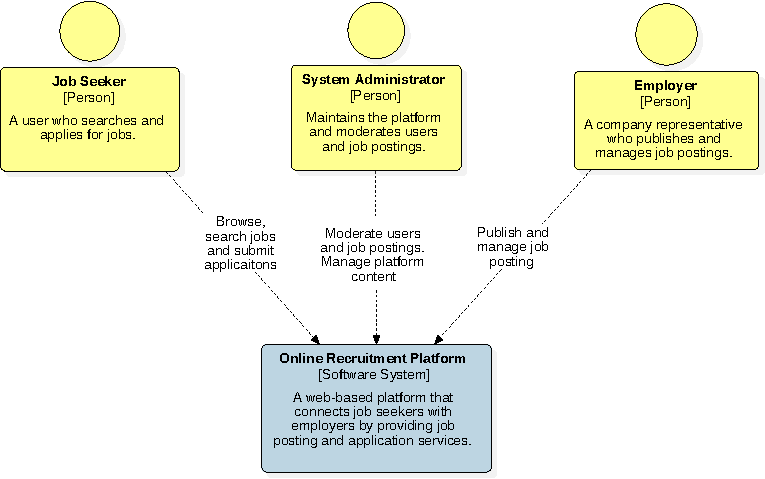
\includegraphics[width=0.85\linewidth]{diagrams/exported/C4/C1-System-Context-Diagram-crop.pdf}
	\caption{System Context Diagram.}
	\label{diagram:c1-context}
\end{figure}

As shown in Figure~\ref{diagram:c1-context}, three actors interact with the platform: the Job Seeker browses and applies for jobs, the Employer publishes and manages job postings, and the System Administrator moderates users and platform content. These actors correspond to the roles established in Chapter \ref{chapter:system-analysis}.

\subsection{Container View}
The Container diagram decomposes the system into its major deployable units and shows how they communicate.

\begin{figure}[H]
	\centering
	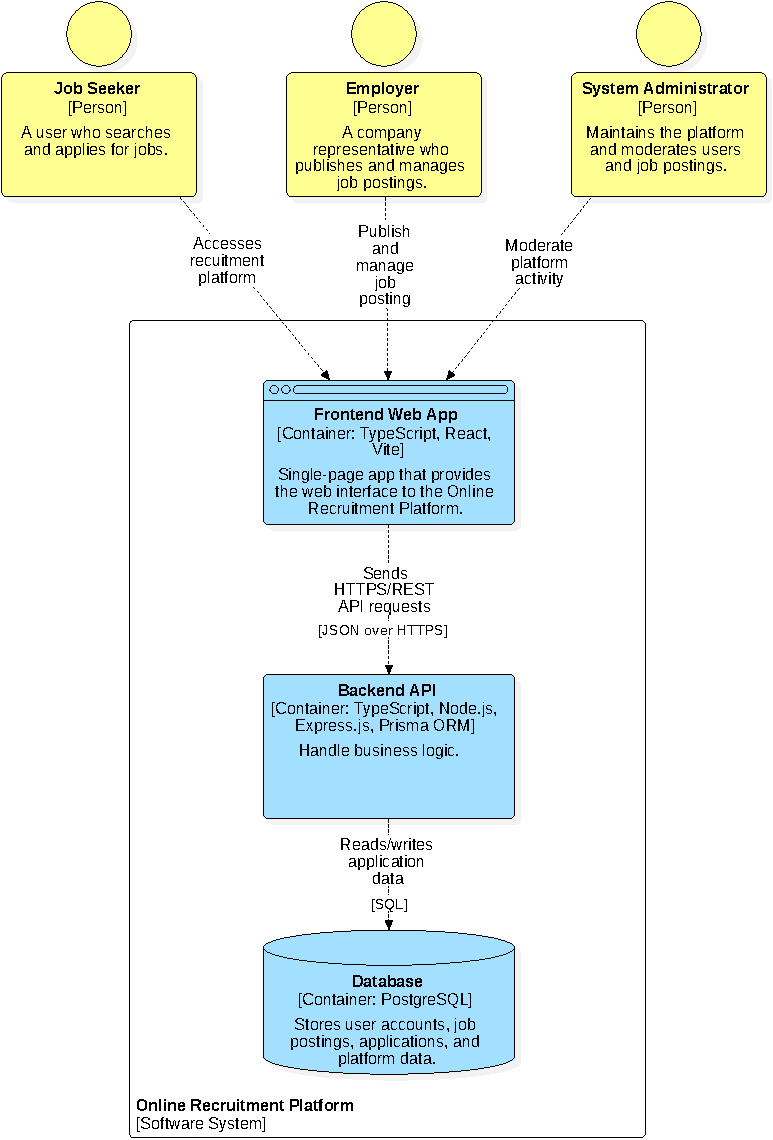
\includegraphics[width=0.75\linewidth]{diagrams/exported/C4/C2-Container-Diagram-crop.pdf}
	\caption{Container Diagram.}
	\label{diagram:c2-container}
\end{figure}

As illustrated in Figure~\ref{diagram:c2-container}, the system consists of three containers:

\begin{itemize}
	\item The \textbf{Frontend Web App} is a React single-page application that renders the user interface.
	\item The \textbf{Backend API} is a Node.js/Express service, built with TypeScript and Prisma ORM, that implements all business logic and exposes it as a REST API.
	\item The \textbf{Database} is a PostgreSQL instance that persists user accounts, job postings, applications, and other platform data.
\end{itemize}

The Frontend communicates with the Backend over HTTPS using JSON, and the Backend communicates with the Database using SQL through Prisma.

\subsection{Component View: Frontend}
The Frontend component diagram decomposes the Frontend Web App container into its internal building blocks.

\begin{figure}[H]
	\centering
	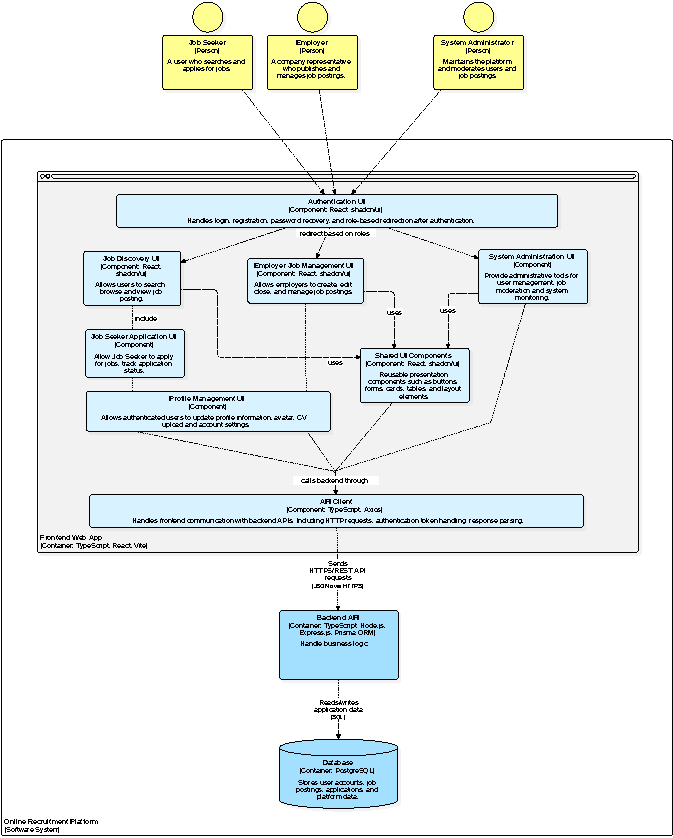
\includegraphics[width=\linewidth]{diagrams/exported/C4/C3-Component-Diagram-(FE)-crop.pdf}
	\caption{Frontend Component Diagram.}
	\label{diagram:c3-frontend}
\end{figure}

As shown in Figure~\ref{diagram:c3-frontend}, the frontend is organized around role-oriented feature components:

\begin{itemize}
	\item The \textbf{Job Seeker Application UI} supports job application submission and status tracking.
	\item The \textbf{Profile Management UI} manages personal information, avatar, and resumes.
	\item The \textbf{Employer Job Management UI} supports company and job posting management.
	\item The \textbf{Authentication UI} handles login, registration, and role-based redirection.
	\item The \textbf{Job Discovery UI} supports job browsing and company profile viewing.
\end{itemize}

All feature components reuse a common Shared UI Components library and communicate with the backend exclusively through a centralized API Client, which handles HTTP requests, authentication tokens, and response parsing.

\subsection{Component View: Backend}
The Backend component diagram decomposes the Backend API container into functional components that implement the platform's business capabilities.

\begin{figure}[H]
	\centering
	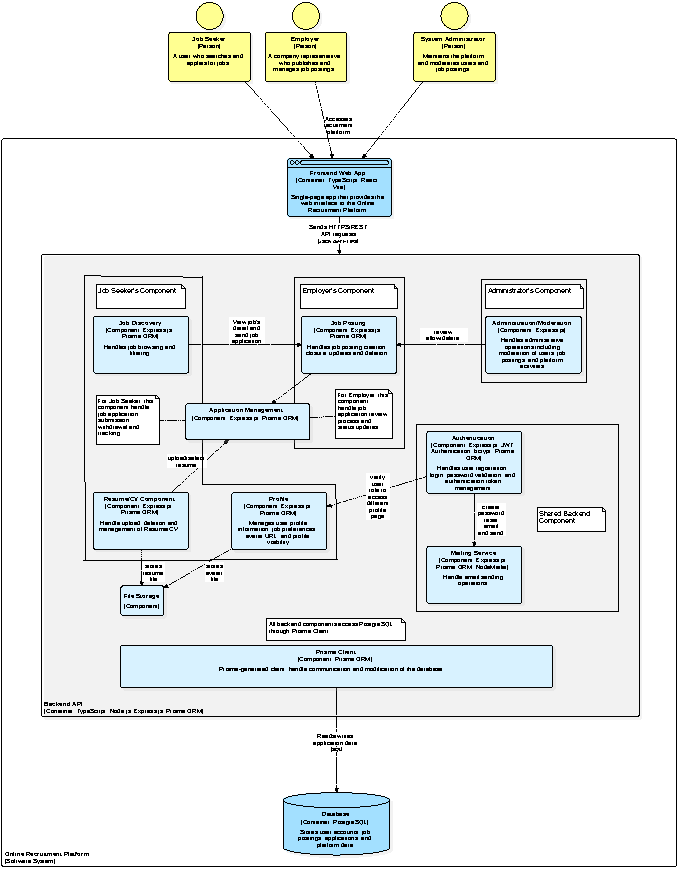
\includegraphics[width=\linewidth]{diagrams/exported/C4/C3-Component-Diagram-(BE)-crop.pdf}
	\caption{Backend Component Diagram.}
	\label{diagram:c3-backend}
\end{figure}

As illustrated in Figure~\ref{diagram:c3-backend}, the backend is organized into role-oriented business components:

\begin{itemize}
	\item The \textbf{Application Management} components support the job seeker's workflow of applying and tracking.
	\item The \textbf{Job Posting} and \textbf{Employer Application Management} components provide employers with job publishing and application review capabilities.
	\item The \textbf{Administration/Moderation} component enables platform administrators to manage users and job postings.
\end{itemize}

Common functionality is centralized in shared infrastructure components. The Authentication component manages user registration, login, and authorization using JWT-based authentication, while the Mailing Service handles email notifications. File assets are stored through the File Storage component.

All business components interact with the PostgreSQL database through the shared \textbf{Prisma Client}, ensuring a consistent data access mechanism across the application.


\section{Database Design}
\label{c4:section:database-design}
The database design defines how the system's persistent data is organized and managed. It identifies the main business entities, their relationships, and the constraints that ensure data consistency. The design follows the principles introduced in Section~\ref{c4:section:design-overview}, particularly data integrity, by using a normalized relational schema with clearly defined primary and foreign key relationships.

\subsection{Entity Relationship Overview}
Figure~\ref{diagram:erd-overview} presents an overview of the complete database schema used by the platform. To improve readability, the overview diagram includes the primary entities, key attributes, and relationships while omitting system-generated fields such as timestamps and audit metadata.

\begin{figure}[H]
	\centering
	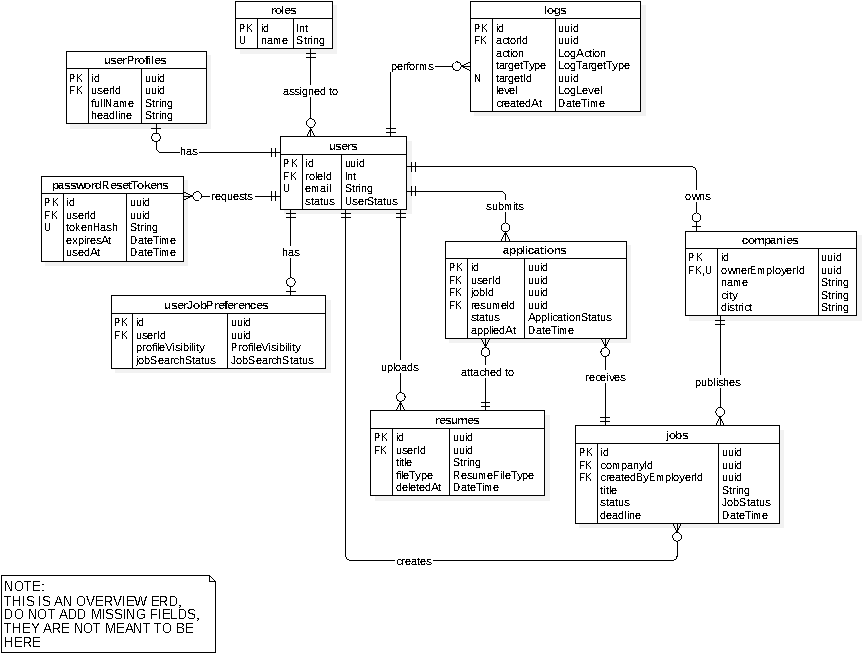
\includegraphics[width=\linewidth]{diagrams/exported/ERD/Overview-ERD-crop.pdf}
	\caption{Entity Relationship Diagram.}
	\label{diagram:erd-overview}
\end{figure}

The remainder of this section details the entity groups that back the two featured modules - the company and job posting domain and the job application domain. The entities supporting the remaining modules are described in the appendix.

\subsection{Company and Job Posting}
Figure~\ref{diagram:erd-company-job} details the entities involved in company and job posting management.

\begin{figure}[H]
	\centering
	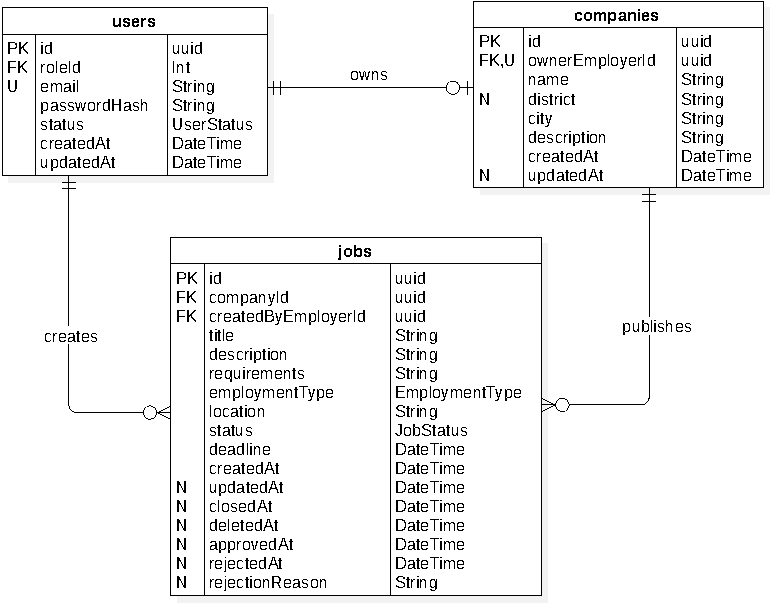
\includegraphics[width=\linewidth]{diagrams/exported/ERD/Company-and-Job-Posting-ERD-crop.pdf}
	\caption{Company and Job Posting Entity Relationship Diagram.}
	\label{diagram:erd-company-job}
\end{figure}

An employer may own multiple companies, but each company belongs to exactly one employer. Similarly, an employer may create multiple job postings, but each job posting is created by exactly one employer. Each job posting belongs to exactly one company, while a company may publish any number of job postings. The status attribute of a job posting tracks its lifecycle - \texttt{PENDING\_APPROVAL}, \texttt{ACTIVE}, \texttt{REJECTED}, \texttt{CLOSED}, \texttt{EXPIRED}, and \texttt{DELETED} - which is the backbone of the Employer Job Management module.

\subsection{Job Application}
Figure~\ref{diagram:erd-job-application} details the entities involved in the job application workflow.

\begin{figure}[H]
	\centering
	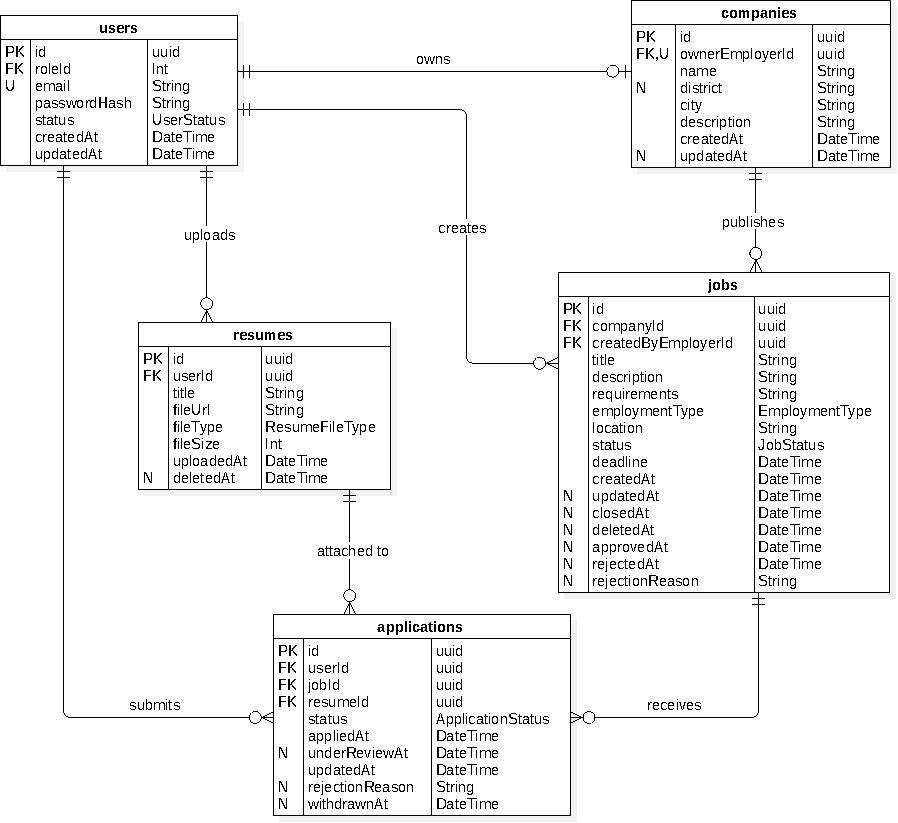
\includegraphics[width=\linewidth]{diagrams/exported/ERD/Job-Application-ERD-crop.pdf}
	\caption{Job Application Entity Relationship Diagram.}
	\label{diagram:erd-job-application}
\end{figure}

A job seeker may upload multiple resumes and submit multiple applications, but each resume and each application belongs to exactly one job seeker. Each application is submitted for exactly one job posting, while a job posting may receive any number of applications. A resume may be attached to multiple applications, but each application references exactly one resume. The application's status attribute - \texttt{SUBMITTED}, \texttt{UNDER\_REVIEW}, \texttt{ACCEPTED}, \texttt{REJECTED}, and \texttt{WITHDRAWN} - records where the application stands in the review process, and a unique constraint on the user-job pair prevents a candidate from applying to the same posting twice.


\section{Backend Design}
\label{c4:section:backend-design}
This section details the internal design of the Backend API container introduced in Section~\ref{c4:section:system-architecture}. It first describes the project structure and shared infrastructure common to all modules, then presents the two featured business modules following the same template: an introduction, a class diagram, and a design explanation. The class diagrams of the remaining modules are presented in the appendix.

\subsection{Backend Project Structure}
\label{c4:subsection:backend-structure}
The backend source code is organized as follows:

\dirtree{%
	.1 src.
	.2 app.ts.
	.2 server.ts.
	.2 authentication.ts.
	.2 api-external.
	.2 api-internal.
	.2 api-shared.
	.2 email.
	.2 generated.
	.2 lib.
	.2 security.
	.2 utils.
}

Table~\ref{tab:backend-folders} summarizes the purpose of each top-level entry.

\begin{table}[H]
	\centering
	\caption{Backend Project Structure.}
	\label{tab:backend-folders}
	\begin{tabular}{|p{3.2cm}|p{10.8cm}|}
		\hline
		\textbf{Entry} & \textbf{Purpose} \\
		\hline
		
		app.ts, server.ts &
		Wire the Express application: register global middleware and the generated routes, and bootstrap the HTTP server. \\
		\hline
		
		authentication.ts &
		Implements \texttt{expressAuthentication} for tsoa: verifies the JWT on protected routes and rejects banned accounts. \\
		\hline
		
		api-external &
		Implements business modules that expose application functionality to external users through RESTful APIs. \\
		\hline
		
		api-internal &
		Implements internal modules that support administrative and platform management operations. \\
		\hline
		
		api-shared &
		Provides reusable guards and logic shared across multiple business domains to reduce duplication. \\
		\hline
		
		email &
		Wraps the mail transport and holds transactional email templates. \\
		\hline
		
		generated &
		Contains files generated by tsoa during the build and should not be modified manually. \\
		\hline
		
		lib &
		Maintains shared library instances and application-wide configurations used by multiple modules. \\
		\hline
		
		security &
		Defines the \texttt{CurrentUser} type that carries the authenticated user's identifier and role into services. \\
		\hline
		
		utils &
		Provides general-purpose utilities such as \texttt{HttpError}, \texttt{PasswordHasher}, \texttt{JwtService}, \texttt{ResetTokenUtils}, and \texttt{FileStorageService}. \\
		\hline
		
	\end{tabular}
\end{table}

\subsection{Shared Backend Components}
\label{c4:subsection:shared-backend-components}
A small set of reusable infrastructure components is shared across all business modules, avoiding duplication and ensuring consistent behavior.

\begin{itemize}
	\item JWT Authentication: issues and verifies signed JSON Web Tokens carrying the user's identifier and role, and is enforced through the \texttt{expressAuthentication} hook on protected routes.
	\item Role Guards: helpers such as \texttt{assertJobSeeker} and \texttt{assertEmployer} reject requests from users who lack the required role, applied as the first step of every service method.
	\item HttpError: a uniform error type carrying an HTTP status and message, translated into the proper JSON error response.
	\item Prisma Client: the generated ORM client, instantiated once in \texttt{lib/prisma.ts} and imported by services for all database access.
	\item File Storage: abstracts file persistence behind a common interface, used for avatar and resume uploads.
	\item Email Service: wraps NodeMailer to send transactional emails, such as password reset notifications.
	\item PasswordHasher and ResetTokenUtils: wrap BCrypt and token generation for credential handling and password recovery.
\end{itemize}

\subsection{Job Application Module}
\label{c4:subsection:job-application-module}
The Job Application Module lets job seekers apply to active job postings using one of their resumes, view their own submitted applications, and withdraw an application while it is still eligible. It resides in \texttt{api-external}, and every endpoint requires both a valid JWT and the \texttt{JOB\_SEEKER} role.

\subsubsection{Class Diagram}
Figure~\ref{diagram:class-job-application} presents the class diagram of the Job Application Module.

\begin{figure}[H]
	\centering
	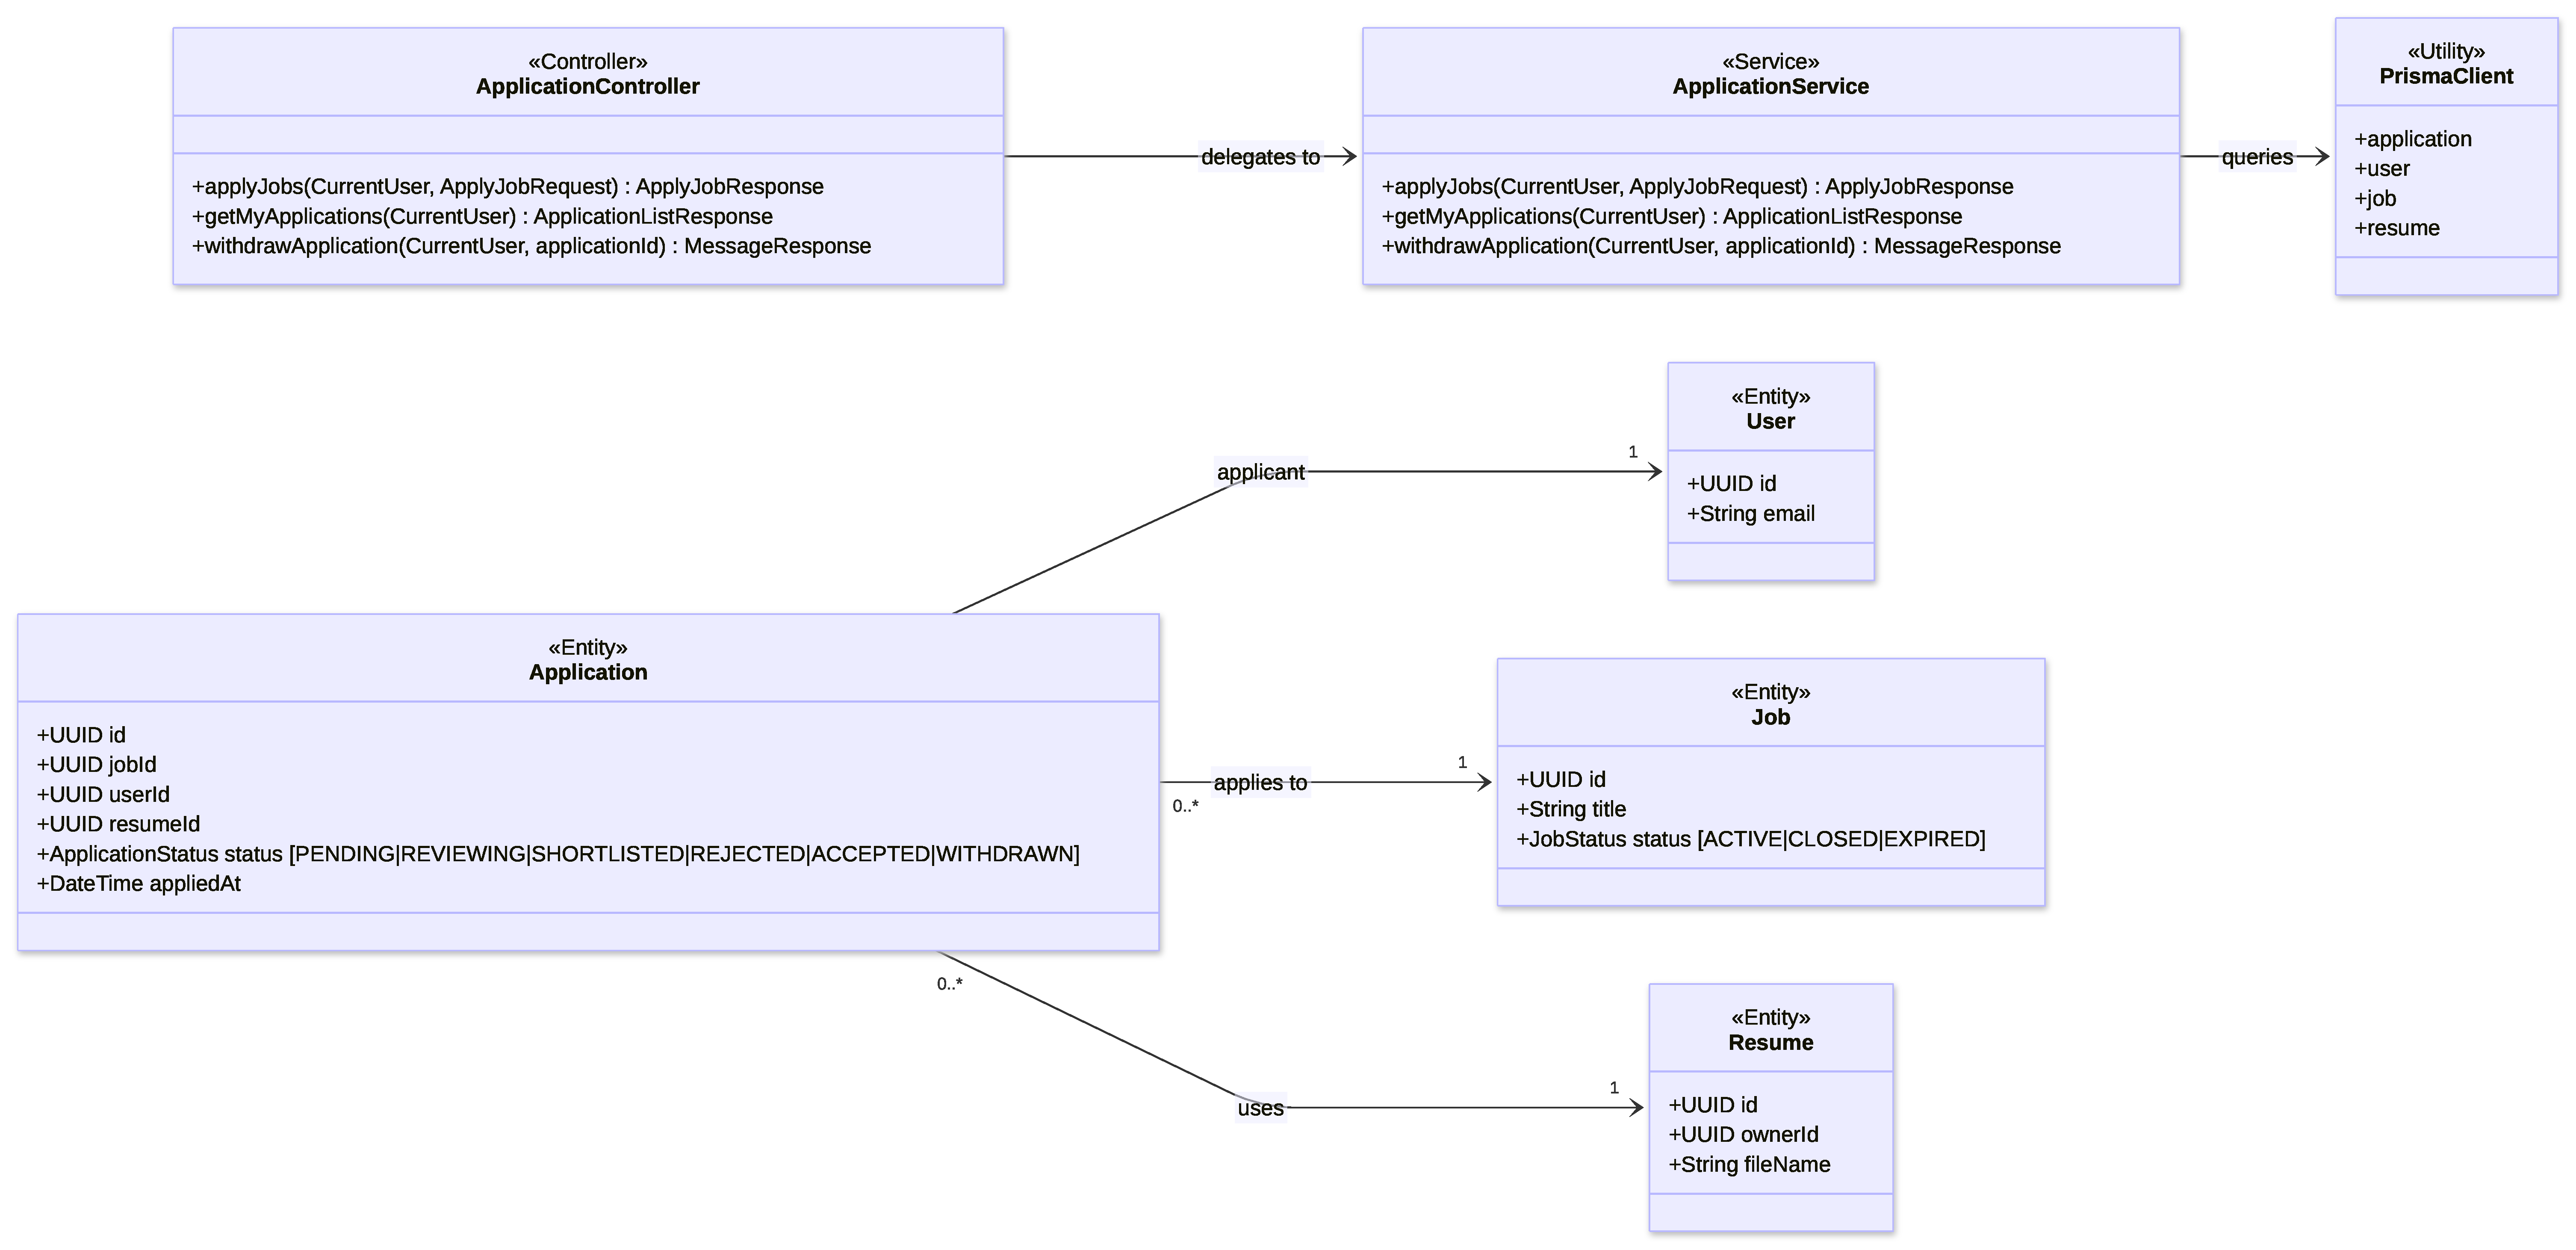
\includegraphics[width=\linewidth]{diagrams/exported/5JobSeeker/JobApplication-Class-Diagram.pdf}
	\caption{Job Application Module Class Diagram.}
	\label{diagram:class-job-application}
\end{figure}

\subsubsection{Design Explanation}
Following the thin controller, rich service principle, ApplicationController exposes three REST endpoints and delegates each directly to a matching method on ApplicationService, without containing business logic itself. ApplicationService depends on the shared PrismaClient, which queries the User, Job, Resume, and Application entities whose relationships are detailed in Figure~\ref{diagram:erd-job-application}.

Every ApplicationService method begins with the same guard: the caller must hold the \texttt{JOB\_SEEKER} role, otherwise the request is rejected. Beyond this shared guard, each method implements one use case:

\begin{itemize}
	\item applyJob verifies that the referenced job exists and is \texttt{ACTIVE}, that the referenced resume exists and belongs to the caller, and that no prior application exists for the same job and user pair, before creating the application with an initial status of \texttt{SUBMITTED}.
	\item getMyApplications returns all applications submitted by the caller, joining through the related job and company to return a flattened summary alongside each application's status and submission date.
	\item withdrawApplication verifies that the application belongs to the caller and is still in \texttt{SUBMITTED} status, rejecting the request once it has moved further along the review process, then updates its status to \texttt{WITHDRAWN} and records the withdrawal timestamp.
\end{itemize}

\subsection{Employer Job Management Module}
\label{c4:subsection:employer-job-module}
The Employer Job Management Module covers the capabilities exposed to employers: managing their company profile, managing the lifecycle of their job postings, and reviewing submitted applications. Together with the Job Application Module, it forms the complete round trip of a recruitment event studied in this thesis.

\subsubsection{Class Diagram}
Figures~\ref{diagram:class-company-profile}, \ref{diagram:class-job-posting}, and \ref{diagram:class-employer-application} present the class diagrams of the Employer Job Management Module.

\begin{figure}[H]
	\centering
	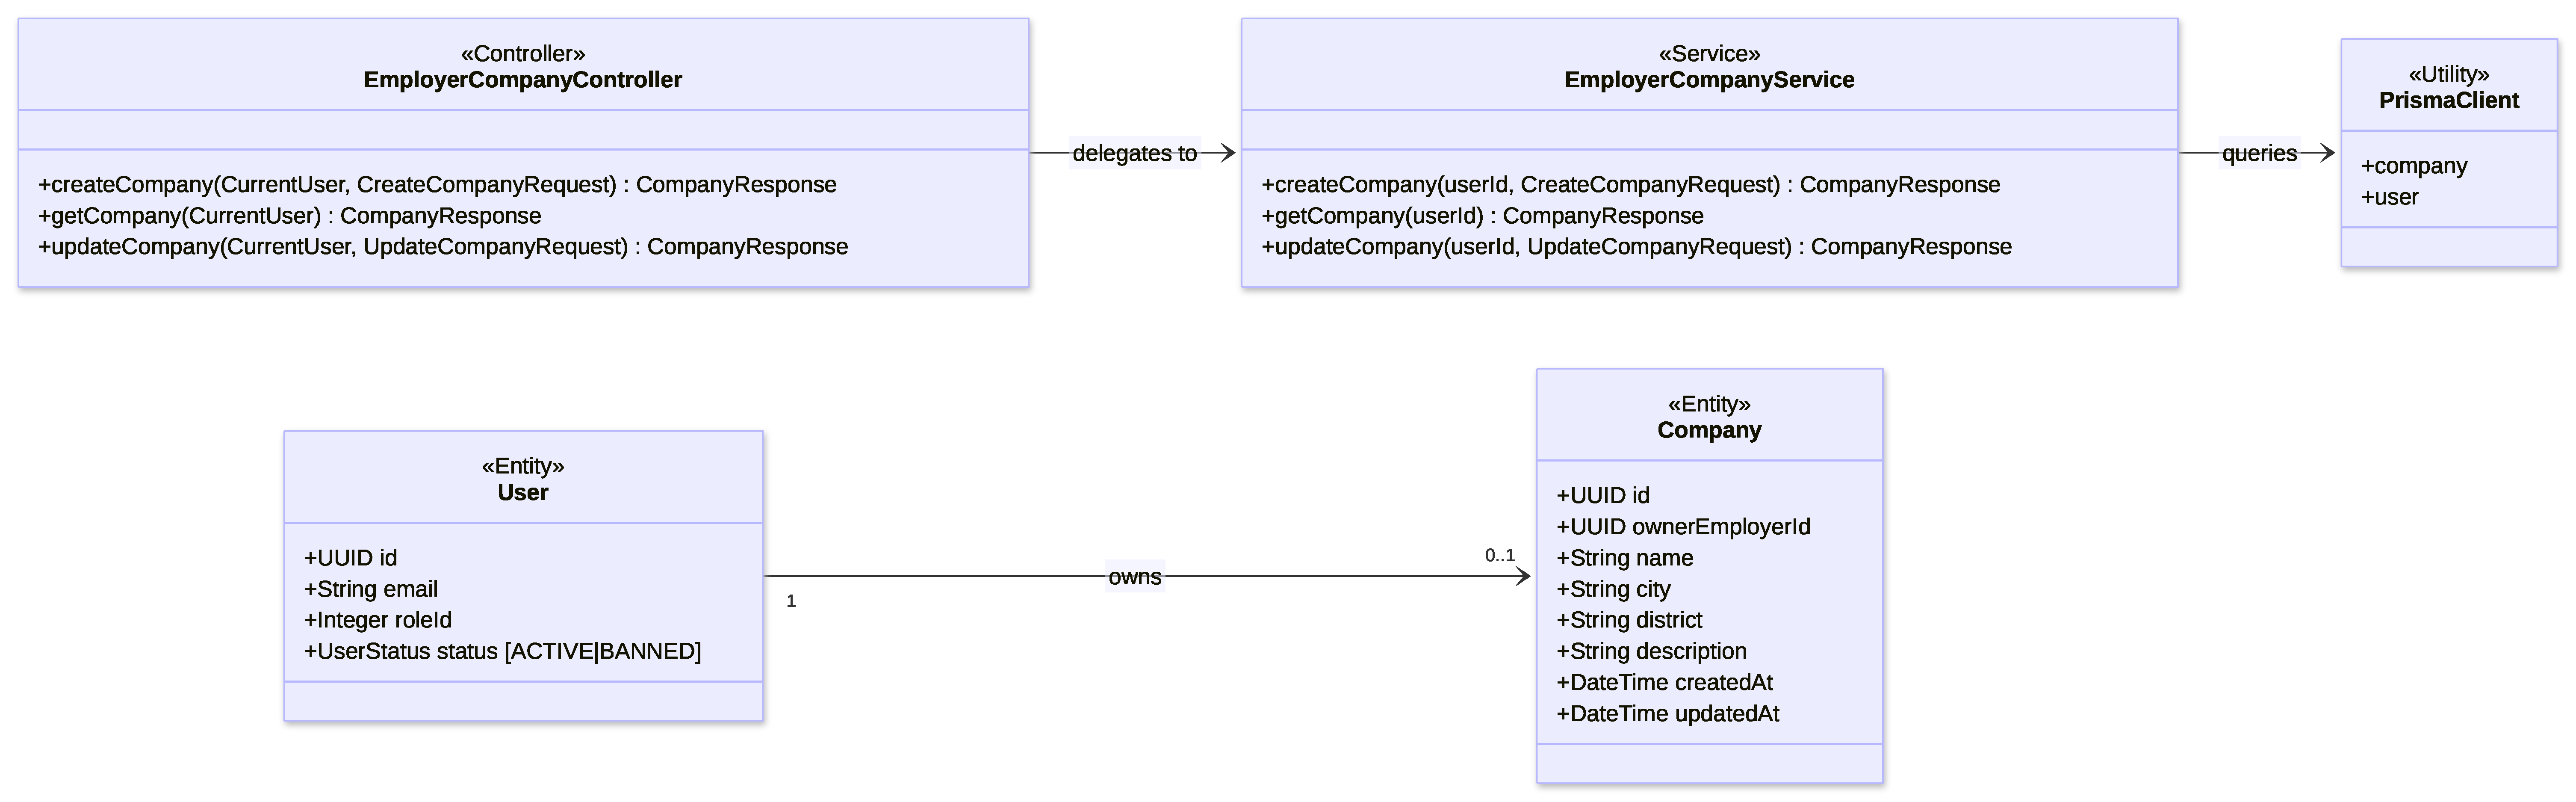
\includegraphics[width=\linewidth]{diagrams/exported/6Employer/CompanyProfileCreation-Class-Diagram.pdf}
	\caption{Company Profile Management Class Diagram.}
	\label{diagram:class-company-profile}
\end{figure}

\begin{figure}[H]
	\centering
	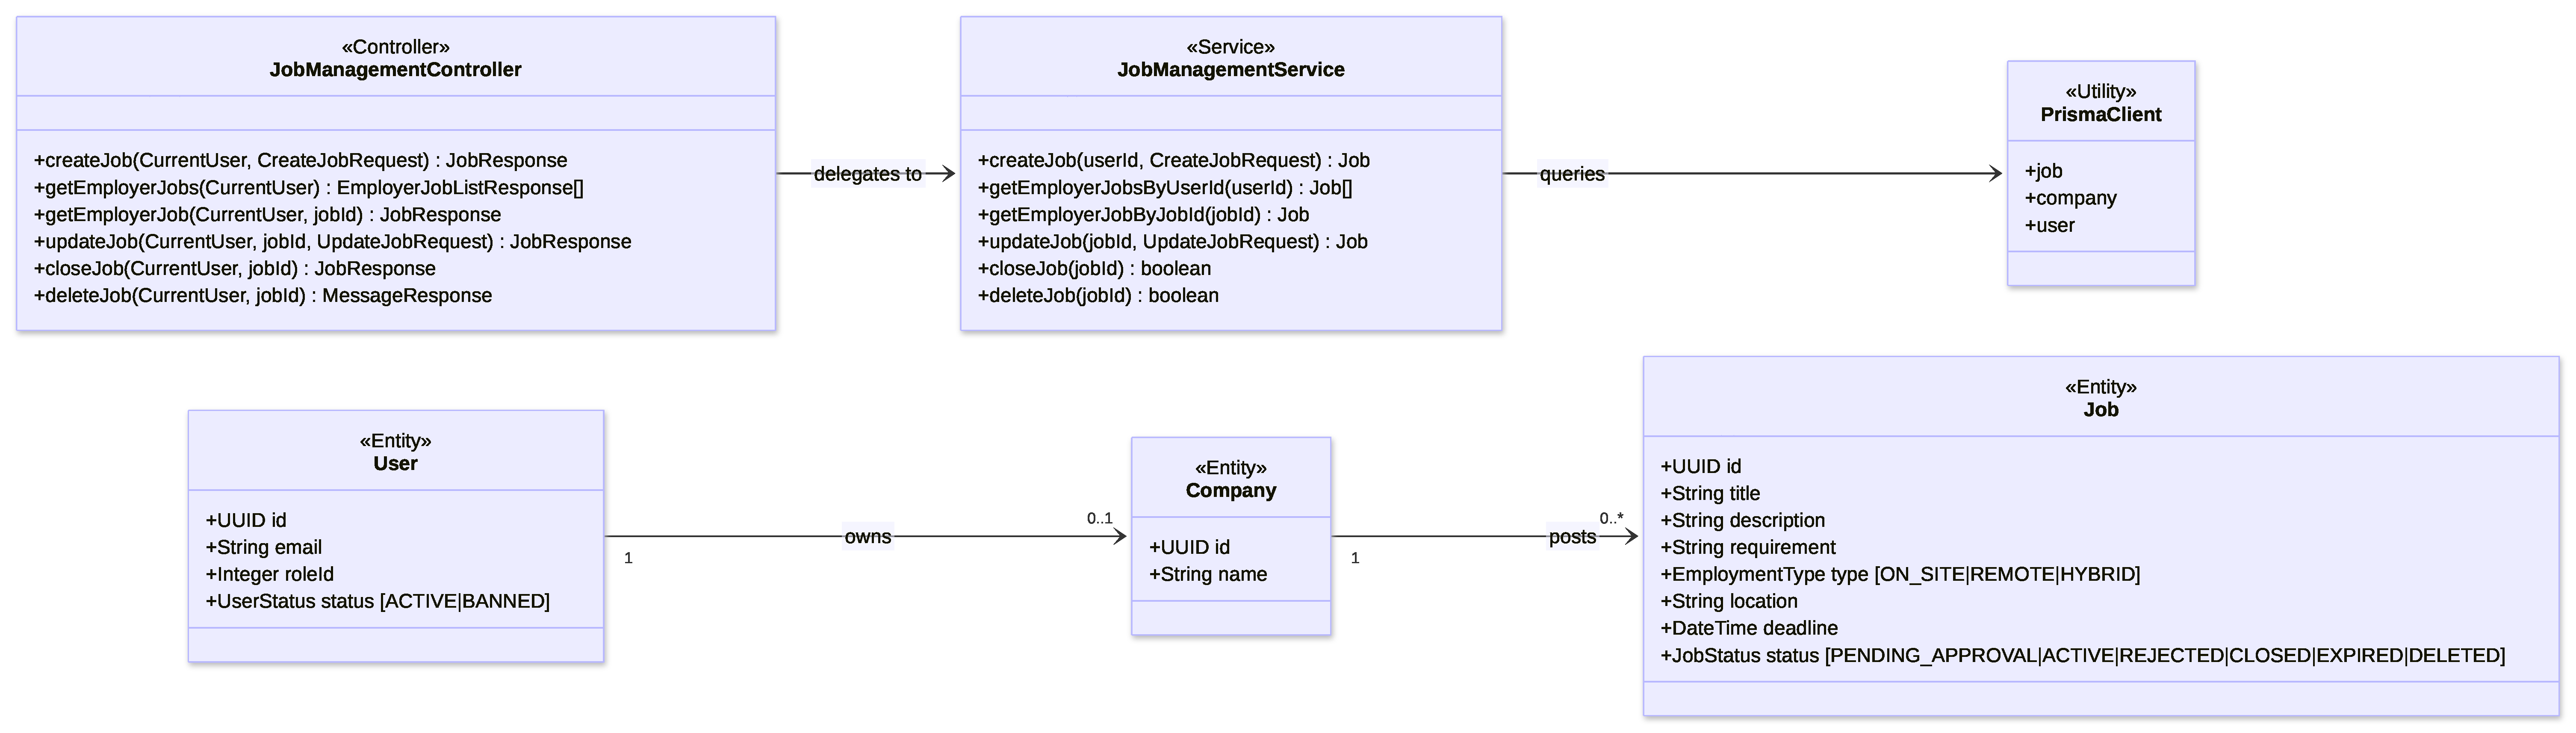
\includegraphics[width=\linewidth]{diagrams/exported/6Employer/JobPostingManagement-Class-Diagram.pdf}
	\caption{Job Posting Management Class Diagram.}
	\label{diagram:class-job-posting}
\end{figure}

\begin{figure}[H]
	\centering
	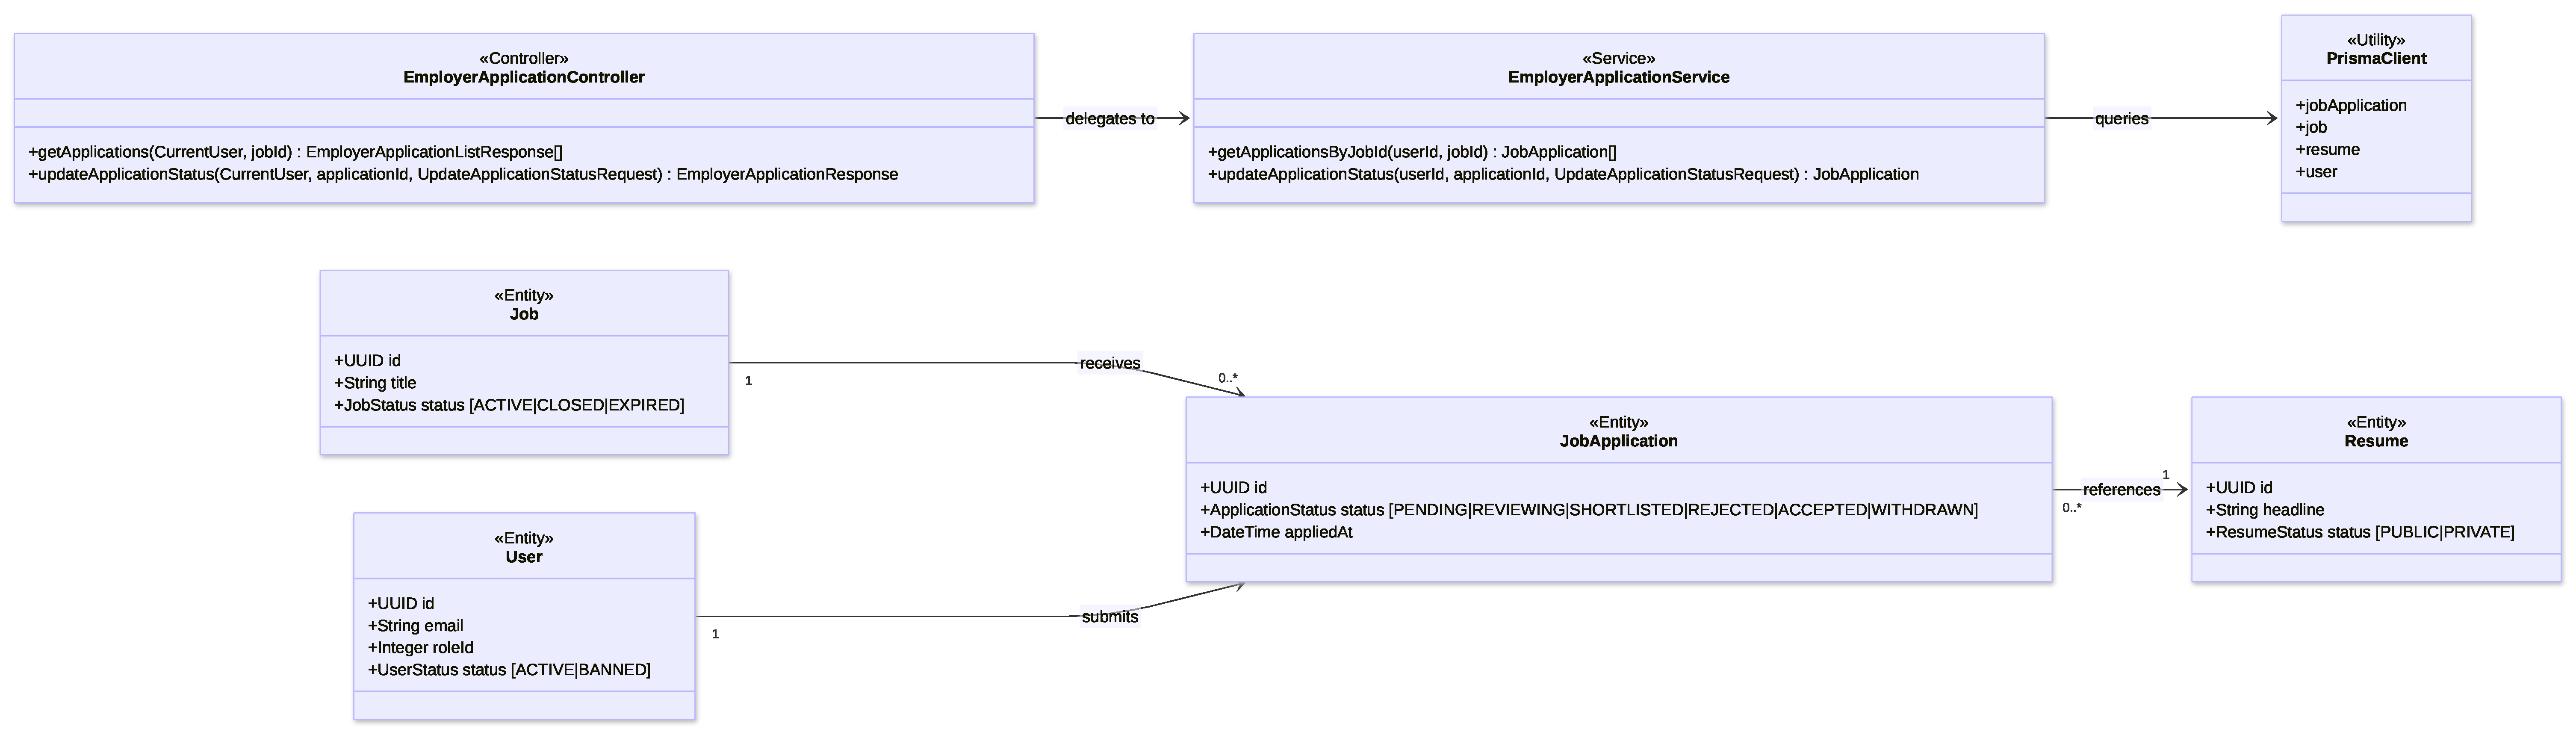
\includegraphics[width=\linewidth]{diagrams/exported/6Employer/EmployerApplicationManagement-Class-Diagram.pdf}
	\caption{Employer Application Management Class Diagram.}
	\label{diagram:class-employer-application}
\end{figure}

\subsubsection{Design Explanation}
Across all three diagrams, each Controller delegates directly to a matching Service method, with no business logic in the controller itself, and each Service depends on the shared PrismaClient and the \texttt{assertEmployer} role guard.

\paragraph{Company Profile Management:}
EmployerCompanyController exposes createCompany, getCompany, and updateCompany, delegated to EmployerCompanyService. An employer owns at most one company, so none of these operations take a company identifier; the owning employer is instead resolved from the authenticated user.

\paragraph{Job Posting Management:}
JobManagementController exposes the full lifecycle of a job posting: createJob, getEmployerJobs, getEmployerJob, updateJob, closeJob, reopenJob, and deleteJob, delegated to JobManagementService. The Job status attribute includes \texttt{PENDING\_APPROVAL} and \texttt{REJECTED}, reflecting that newly created and edited postings are subject to moderation before becoming publicly visible.

\paragraph{Application Review:}
EmployerApplicationController exposes getJobApplications, getJobApplicationDetail, putApplicationUnderReview, and updateApplicationStatus, delegated to EmployerApplicationService. This complements the \texttt{SUBMITTED} and \texttt{WITHDRAWN} transitions initiated by the job seeker: here, the employer moves an application through the remaining \texttt{UNDER\_REVIEW}, \texttt{ACCEPTED}, and \texttt{REJECTED} statuses.


\section{Frontend Design}
\label{c4:section:frontend-design}

The frontend is a React single-page application. Pages are grouped in feature folders that mirror the backend module structure, so a feature can be traced end to end. Reusable UI is separated into \texttt{ui-shared/}. Routing is role-based: \texttt{RequireAuth} guards wrap route groups so that a Job Seeker-only area and an Employer-only area are rendered only for the matching role. All API calls go through a client generated from the backend's OpenAPI specification, so the request and response types used by the pages always match the backend contract.

\subsection{Job Application UI}
The Job Application UI consists of two pages. The apply page, \texttt{ApplyJobPage} at \texttt{/jobs/:jobId/apply}, loads the chosen posting and the user's resumes, presents the job summary together with a \texttt{ResumeSelector}, and submits the selected resume. The submit errors are handled by HTTP status: a \texttt{409} reports that the user already applied, a \texttt{401} prompts re-login, and a \texttt{403} reports that only job seekers can apply. The tracking page, \texttt{MyApplicationsPage} at \texttt{/applications}, lists the user's applications through \texttt{ApplicationCard} components that show the posting, company, status badge, and submission date. Withdrawing an application is confirmed through a shared \texttt{ConfirmationDialog}; on success the card status is updated locally to \texttt{WITHDRAWN}.

\subsection{Employer Job Management UI}
The Employer Job Management UI covers two pages. \texttt{PostJobPage} at \texttt{/employer/jobs/new} collects a posting through \texttt{JobPostingForm}, which validates each field and converts the chosen calendar date into an ISO deadline at the end of that day via the shared deadline helper. \texttt{MyJobPostingsPage} at \texttt{/employer/jobs} lists the employer's postings with a \texttt{JobStatusBadge}; close, re-open, and delete actions each require confirmation in a \texttt{ConfirmationDialog} and the list is refreshed after the mutation. The company profile page, \texttt{MyCompanyPage}, manages the employer's company. The application review screens that use the employer application review endpoints are still in progress at the time of writing.

\section{Summary}
\label{c4:section:summary}

This chapter presented the technical design of the platform. The system follows a layered, feature-oriented architecture split into a React frontend, a Node.js/Express API, and a PostgreSQL database. The database design centered on the entity groups that serve the two featured modules: company and job posting, and job application. The backend design introduced the project structure, the shared infrastructure components, and the class-level design of the Job Application and Employer Job Management modules. The frontend design described the page structure for both featured modules. The next chapter describes how this design was realized in code.